\documentclass{article}

\title{Extended zCall}
\author{Iain Bancarz\\
  Wellcome Trust Sanger Institute\\
  \texttt{ib5@sanger.ac.uk}}
\date{3 April 2013}

\usepackage{graphicx}
\usepackage{placeins}
\usepackage{url}

\begin{document}

\maketitle

\section{Introduction}

zCall is a rare variant caller for array-based genotyping, developed by JI Goldstein et al.\ \cite{gold}. This document describes a major extension of zCall, intended to support inclusion in the Wellcome Trust Sanger Institute Genotyping Pipeline \cite{wtsi-gp, wtsi-zcall}.

\section{Summary of new features}

\begin{itemize}
\item \textbf{Calibration:} Definition of metrics and a heuristic for evaluating candidate zscore values; see Section \ref{sec:calib}.
\item \textbf{Automation:} Automated implementation of zCall, invoked by either a single command-line script, or four separate scripts to enable parallelization.
\item \textbf{Logging:} Intermediate metadata, such as results of threshold evaluation, is saved in .json format files. Results of applying zCall to previously uncalled genotypes are summarized in a file \texttt{zcall\_log.json}.
\item \textbf{Plink output:} Output in the Plink genotyping data format, in either binary or non-binary form \cite{plink, plink-soft}.
\item \textbf{Pydoc:} The \texttt{createDocs.py} script uses Python's Pydoc module to generate HTML documentation for zCall code and its dependencies.
\item \textbf{Unit tests:} Using the standard Python unit test suite, in \texttt{src/test/test.py}.
\end{itemize}

\section{Calibration}
\label{sec:calib}

The zCall method requires the choice of a threshold known as the `zscore'. This threshold is the number of standard deviations away from the mean of genotyping intensity clusters, to be used as a boundary between genotype calls. Goldstein et al.\ recommended a zscore of 7 as a suitable default value \cite{gold}. A threshold of 7 standard deviations by definition will affect very few calls, but this is appropriate, as zCall is intended as a post-processing step applied to a small subset of `badly behaved' data points.

Goldstein et al.\ note that the choice of zscore can be informed by comparing the outputs of zCall and another caller. We now present a systematic procedure for evaluating candidate zscores on a given test data set.

\subsection{Metrics}

In production, zCall is applied to data points which failed to be called by a `default caller'. The default caller is typically Illumina's GenCall software, but may also be a third-party package such as Illuminus or GenoSNP \cite{genosnp, illuminus}.

For an input data point $x$, let $d(x)$ be the call under a default caller and  $Z(x,k)$ be the call made by zCall with a zscore of $k$. Let $\phi$ represent a no-call. We define two metrics which may be used to assess a given zscore on a set of test data:
\begin{itemize}
\item \textbf{Concordance:} The proportion of points $x$ such that $d(x) \neq \phi$ and $d(x) = Z(x,k)$. These points are called by both callers, and are given the same call by each.
\item \textbf{Gain:} The proportion of points $x$ such that $d(x) = \phi$ and $Z(x,k) \neq \phi$. These points are called by zCall, but not by the default caller.
\end{itemize}

\subsection{Heuristic for choosing a zscore}

Intuitively, we would like to maximize both concordance and gain.  Assuming that our default caller is reasonably good at finding the true genotype, we would like zCall to agree with it. Conversely, we would like as many no-calls as possible to be `rescued' by zCall.

The gain is maximized where $z=0$ and will decrease as $z$ increases; the higher the value of $z$, the greater the volume of intensity space which zCall will designate for no-calls. Concordance is likely to be low for very low or very high values of $z$, and maximized for some intermediate value. 

Suppose that we have evaluated the concordance and gain for a range of candidate zscores. We define the following heuristic for choosing a candidate zscore $z$:

\begin{quote}Choose the smallest value of $z$ such that concordance is greater than gain; or if no such $z$ is in the set of candidates, the value of $z$ with the greatest concordance.
\end{quote}

The above heuristic is simple to automate, and has been implemented in the zCall extended software. It can be thought of as re-calling all data points with multiple zscores as a first pass, after which zcall is applied with the chosen zscore to re-call any no-calls.

Evaluating candidate thresholds with this heuristic requires much more computation than the actual application of zcall. However, it is straightforward to parallelize by evaluating different zscores and subsets of samples on different processes; this will be implemented in the WTSI Genotyping Pipeline \cite{wtsi-gp}. 

In addition, zCall does not require highly intensive computation, and a single processor is easily sufficient to calibrate and call for medium-sized test datasets such as the one in Section \ref{sec:evaluation}.  For larger datasets, one may use parallel processing, or simply evaluate candidate zscores on a representative subset of the available samples.

\subsection{Evaluation on test data}
\label{sec:evaluation}

The heuristic has been found to achieve good results on test data. In assessment on a set of 94 samples genotyped with the Illumina HumanExome-12v1 beadchip, the criterion was met at $z=7$, with concordance and gain of 96.9\% and 96.3\% respectively. Concordance and gain for a range of zscores on this dataset are shown in Figure \ref{fig:zscores}.

\begin{figure}[t]
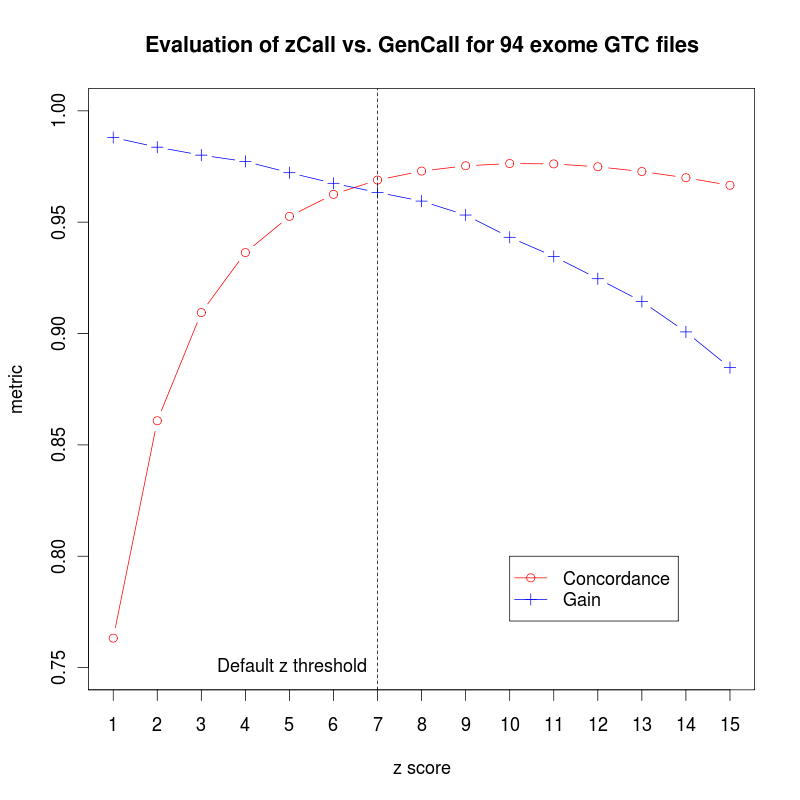
\includegraphics[width=1.0\textwidth]{concordance_gain_means.png}
\caption{Concordance and gain metrics on a test dataset.}
\label{fig:zscores}
\end{figure}

In this case, the chosen zscore happened to equal the default suggested by Goldstein et al. In other choices of test dataset, the zscore chosen by the heuristic was typically between 6 and 8. The range of zscores to evaluate for production will depend on the preferences and computational resources of the user, but a range of 4 to 10 may be appropriate.

\section{Conclusion and further reading}

This document has summarized changes introduced in extended zcall, and presented metrics and a heuristic for choosing a zscore threshold.

See the \texttt{README}, \texttt{README\_prototype}, and \texttt{README\_extended} files, in the top-level directory of the zCall repository, for additional details.  \texttt{README\_extended} has instructions for installation and usage of extended zCall. The  \texttt{updates.txt} file contains a history of changes. Tests are documented in \texttt{src/test/README}.

\FloatBarrier

\begin{thebibliography}{9}

\bibitem{genosnp} A Variational Bayes within-sample SNP genotyping algorithm that does not require a reference population. Giannoulatou E, Yau C, Colella S, Ragoussis J, Holmes CC. Bioinformatics. 2008 Oct 1;24(19):2209-14

\bibitem{gold}
Goldstein JI, Crenshaw A, Carey J, Grant GB, Maguire J, Fromer M, O'Dushlaine C, Moran JL, Chambert K, Stevens C; Swedish Schizophrenia Consortium; ARRA Autism Sequencing Consortium, Sklar P, Hultman CM, Purcell S, McCarroll SA, Sullivan PF, Daly MJ, Neale BM. 
zCall: a rare variant caller for array-based genotyping.
Genetics and population analysis. Bioinformatics 2012 Oct 1;28(19):2543-2545. Epub 2012 Jul 27. PubMed PMID: 22843986.

\bibitem{plink}
Purcell S, Neale B, Todd-Brown K, Thomas L, Ferreira MAR, Bender D, Maller J, Sklar P, de Bakker PIW, Daly MJ \& Sham PC (2007).
PLINK: a toolset for whole-genome association and population-based linkage analysis. American Journal of Human Genetics, 81.

\bibitem{plink-soft}
Purcell S. PLINK software v1.07. \url{http://pngu.mgh.harvard.edu/purcell/plink/}

\bibitem{illuminus} A genotype calling algorithm for the Illumina BeadArray platform. Teo YY, Inouye M, Small KS, Gwilliam R, Deloukas P, Kwiatkowski DP and Clark TG. Bioinformatics 2007;23;20;2741-6

\bibitem{wtsi-gp}
Wellcome Trust Sanger Institute Genotyping Pipeline. \url{https://github.com/wtsi-npg/genotyping} 

\bibitem{wtsi-zcall} 
Wellcome Trust Sanger Institute fork of the zCall repository. \url{https://github.com/wtsi-npg/zcall} 

\end{thebibliography}

\end{document}
